
\section*{Galileo’s Big Shot: From Cannonballs to Inertia}

\textbf{Aristotle (4th century BCE)} had taught that \textbf{heavier objects fall faster} than lighter ones because they have a greater “natural motion.” This belief went unchallenged for centuries—until \textbf{Galileo Galilei (1600s)} decided to put it to the test.

Galileo was fascinated by cannonballs and their curved trajectories. Cannons, a new and powerful weapon in Renaissance warfare, provided a perfect testing ground for the physics of motion.

He made a key observation:

\begin{itemize}
    \item Cannonballs don’t travel in a straight line when fired. Instead, they \textbf{arc downward over time}.
    \item The longer they travel, the \textbf{steeper their descent} becomes.
    \item The path of a cannonball is a \textbf{parabola}—a shape he could describe mathematically.
\end{itemize}

\begin{center}
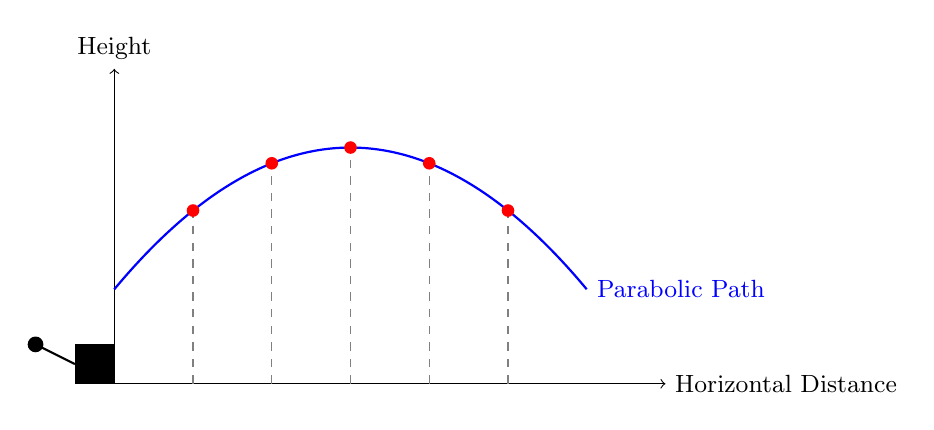
\begin{tikzpicture}
    \draw[->] (0,0) -- (7,0) node[right] {\small Horizontal Distance};
    \draw[->] (0,0) -- (0,4) node[above] {\small Height};
    \fill[black] (-0.5,0) rectangle (0,0.5);
    \draw[thick] (-0.5,0.25) -- (-1,0.5);
    \fill[black] (-1,0.5) circle (0.1);
    \draw[thick, blue, domain=0:6, samples=50, smooth, variable=\x] plot ({\x},{-0.2*(\x-3)*(\x-3)+3}) node[right] {\small Parabolic Path};
    \foreach \x in {1,2,3,4,5} {
        \draw[dashed, gray] (\x,0) -- (\x,{-0.2*(\x-3)*(\x-3)+3});
        \fill[red] (\x,{-0.2*(\x-3)*(\x-3)+3}) circle (0.08);
    }
\end{tikzpicture}
\end{center}

%\subsubsection*{The Physics Behind the Parabola: Motion and Stored Capacity}

%Galileo didn’t use the terms \textbf{kinetic energy} or \textbf{potential energy}—but he stumbled right into them.

When he studied falling bodies, he noticed that something changed with height. A ball at the top of a ramp seemed to have a kind of “stored power,” and when released, it converted that into motion. The steeper the ramp, the faster the ball gained speed.

He called this increasing quantity of motion \textit{impeto}: a kind of internal momentum or urge to move. Today, we’d describe this in terms of energy:

\begin{itemize}
    \item The height of the ball gave it \textbf{potential energy}.
    \item As it fell, that stored capacity was released and turned into \textbf{kinetic energy}.
\end{itemize}

Galileo even calculated that falling bodies obey the equation:
\[
d \propto t^2
\]

This hinted at something being conserved, and the relationship between height and motion that would later become formalized in energy conservation.  However, \textit{Galileo couldn’t yet write the equation \( E_{\text{pot}} = E_{\text{kin}} \), but he saw the tradeoff happen: energy wasn’t just “spent,” it was transformed.}

\begin{figure}[H]
\centering
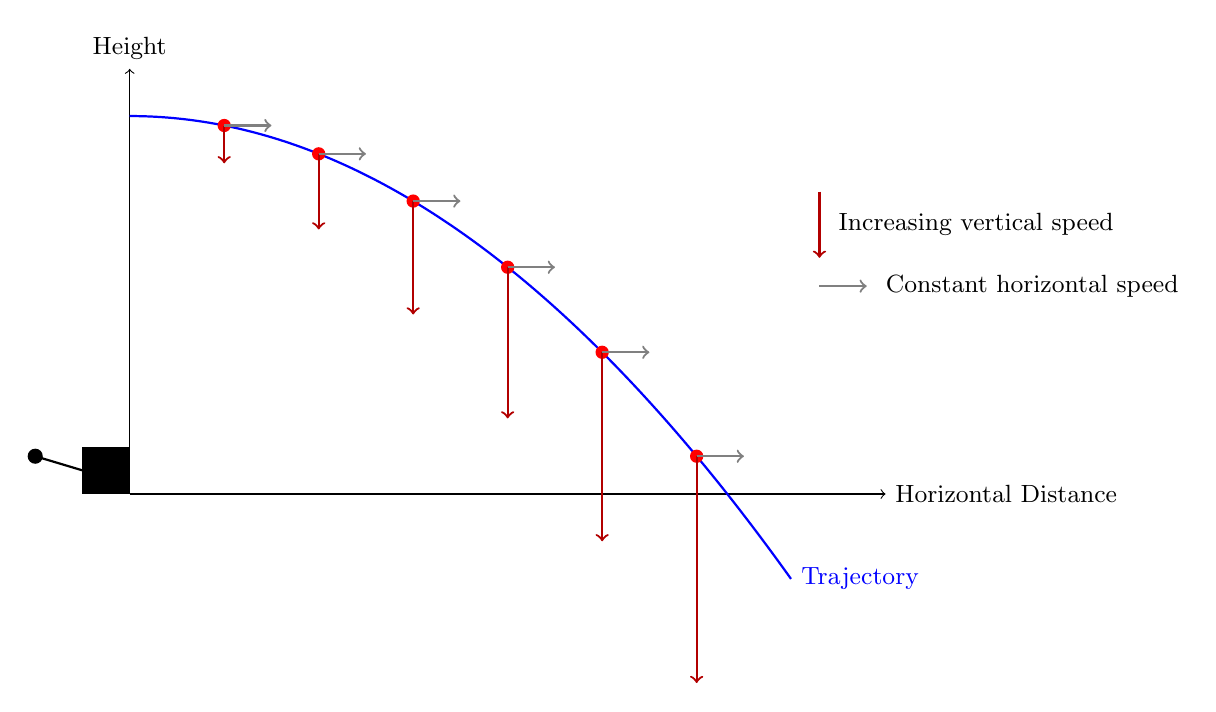
\begin{tikzpicture}[scale=1.2]
    \draw[->] (0,0) -- (8,0) node[right] {\small Horizontal Distance};
    \draw[->] (0,0) -- (0,4.5) node[above] {\small Height};
    \fill[black] (-0.5,0) rectangle (0,0.5);
    \draw[thick] (-0.5,0.25) -- (-1,0.4);
    \fill[black] (-1,0.4) circle (0.08);
    \draw[thick, blue, domain=0:7, smooth, samples=100, variable=\x] 
        plot ({\x}, {4 - 0.1*\x*\x}) node[right] {\small Trajectory};

    \foreach \t in {1,2,3,4,5,6} {
        \pgfmathsetmacro{\y}{4 - 0.1*(\t*\t)}
        \fill[red] (\t, \y) circle (2pt);
        \draw[->, thick, red!70!black] (\t, \y) -- (\t, {\y - 0.4*\t});
    }

    \foreach \t in {1,2,3,4,5,6} {
        \pgfmathsetmacro{\y}{4 - 0.1*(\t*\t)}
        \draw[->, thick, gray] (\t, \y) -- ({\t + 0.5}, \y);
    }

    \draw[->, thick, red!70!black] (7.3,3.2) -- (7.3,2.5);
    \node[right] at (7.4,2.85) {\small Increasing vertical speed};

    \draw[->, thick, gray] (7.3,2.2) -- (7.8,2.2);
    \node[right] at (7.9,2.2) {\small Constant horizontal speed};
\end{tikzpicture}
\caption{\small Galileo described projectile motion as a fusion of constant horizontal motion and vertical acceleration.}
\end{figure}

\subsection{The Inertia Revolution}

Aristotle’s physics said motion required a cause, and objects naturally came to rest. If the Earth were truly spinning, wouldn’t we feel it?

\textbf{But Galileo’s ramp experiments held the answer: inertia.}

\begin{itemize}
    \item Once an object is in motion, it \textbf{stays in motion} unless acted upon.
    \item That meant that if Earth were moving, everything on it would move too.
    \item Like a cannonball in flight: steady horizontal motion + vertical acceleration = parabolic motion.
\end{itemize}


The Scholastics had kept alive Aristotle’s notion that objects possess \textit{potentia}—the potential to act or change. Galileo’s experiments gave that idea a physical form.

\begin{quote}
Height wasn’t just a location; it was stored possibility. Motion wasn’t just a path; it was the release of that possibility. Today, we call them \textbf{potential energy} and \textbf{kinetic energy}.
\end{quote}

\textit{Galileo translated metaphysical potential into physical energy.} And though he never used the word “energy,” he clearly saw the dance between ramp and ball, between height and velocity, and between philosophy and physics.

\begin{figure}[H]
\centering
\begin{tikzpicture}[every node/.style={font=\footnotesize}]

% Panel 1 — Galileo explains inertia
\comicpanel{0}{4}
  {Galileo}
  {Aristotle}
  {\textbf{Galileo:} I rolled a ball down a ramp. The flatter the surface, the longer it moved. I think motion continues unless something stops it.}
  {(0,-0.5)}

% Panel 2 — Aristotle looks unimpressed
\comicpanel{6.5}{4}
  {Aristotle}
  {Galileo}
  {\textbf{Aristotle:} So... you’re saying a rock just keeps moving? On its own? That’s absurd. Motion needs a purpose.}
  {(0,-0.5)}

% Panel 3 — Galileo is confused
\comicpanel{0}{0}
  {Galileo}
  {Aristotle}
  {\textbf{Galileo:} It doesn't need a purpose. It just keeps going. That’s inertia.}
  {(0,0.8)}

% Panel 4 — Aristotle lands the punchline
\comicpanel{6.5}{0}
  {Aristotle}
  {Student}
  {\textbf{Aristotle:} Motion without purpose? Might as well say the rock has free will.}
  {(0,0.8)}

\end{tikzpicture}
\caption{Inertia: the radical idea that objects don’t need permission to keep moving.}
\end{figure}

